\begin{figure}[ht]
    \centering
    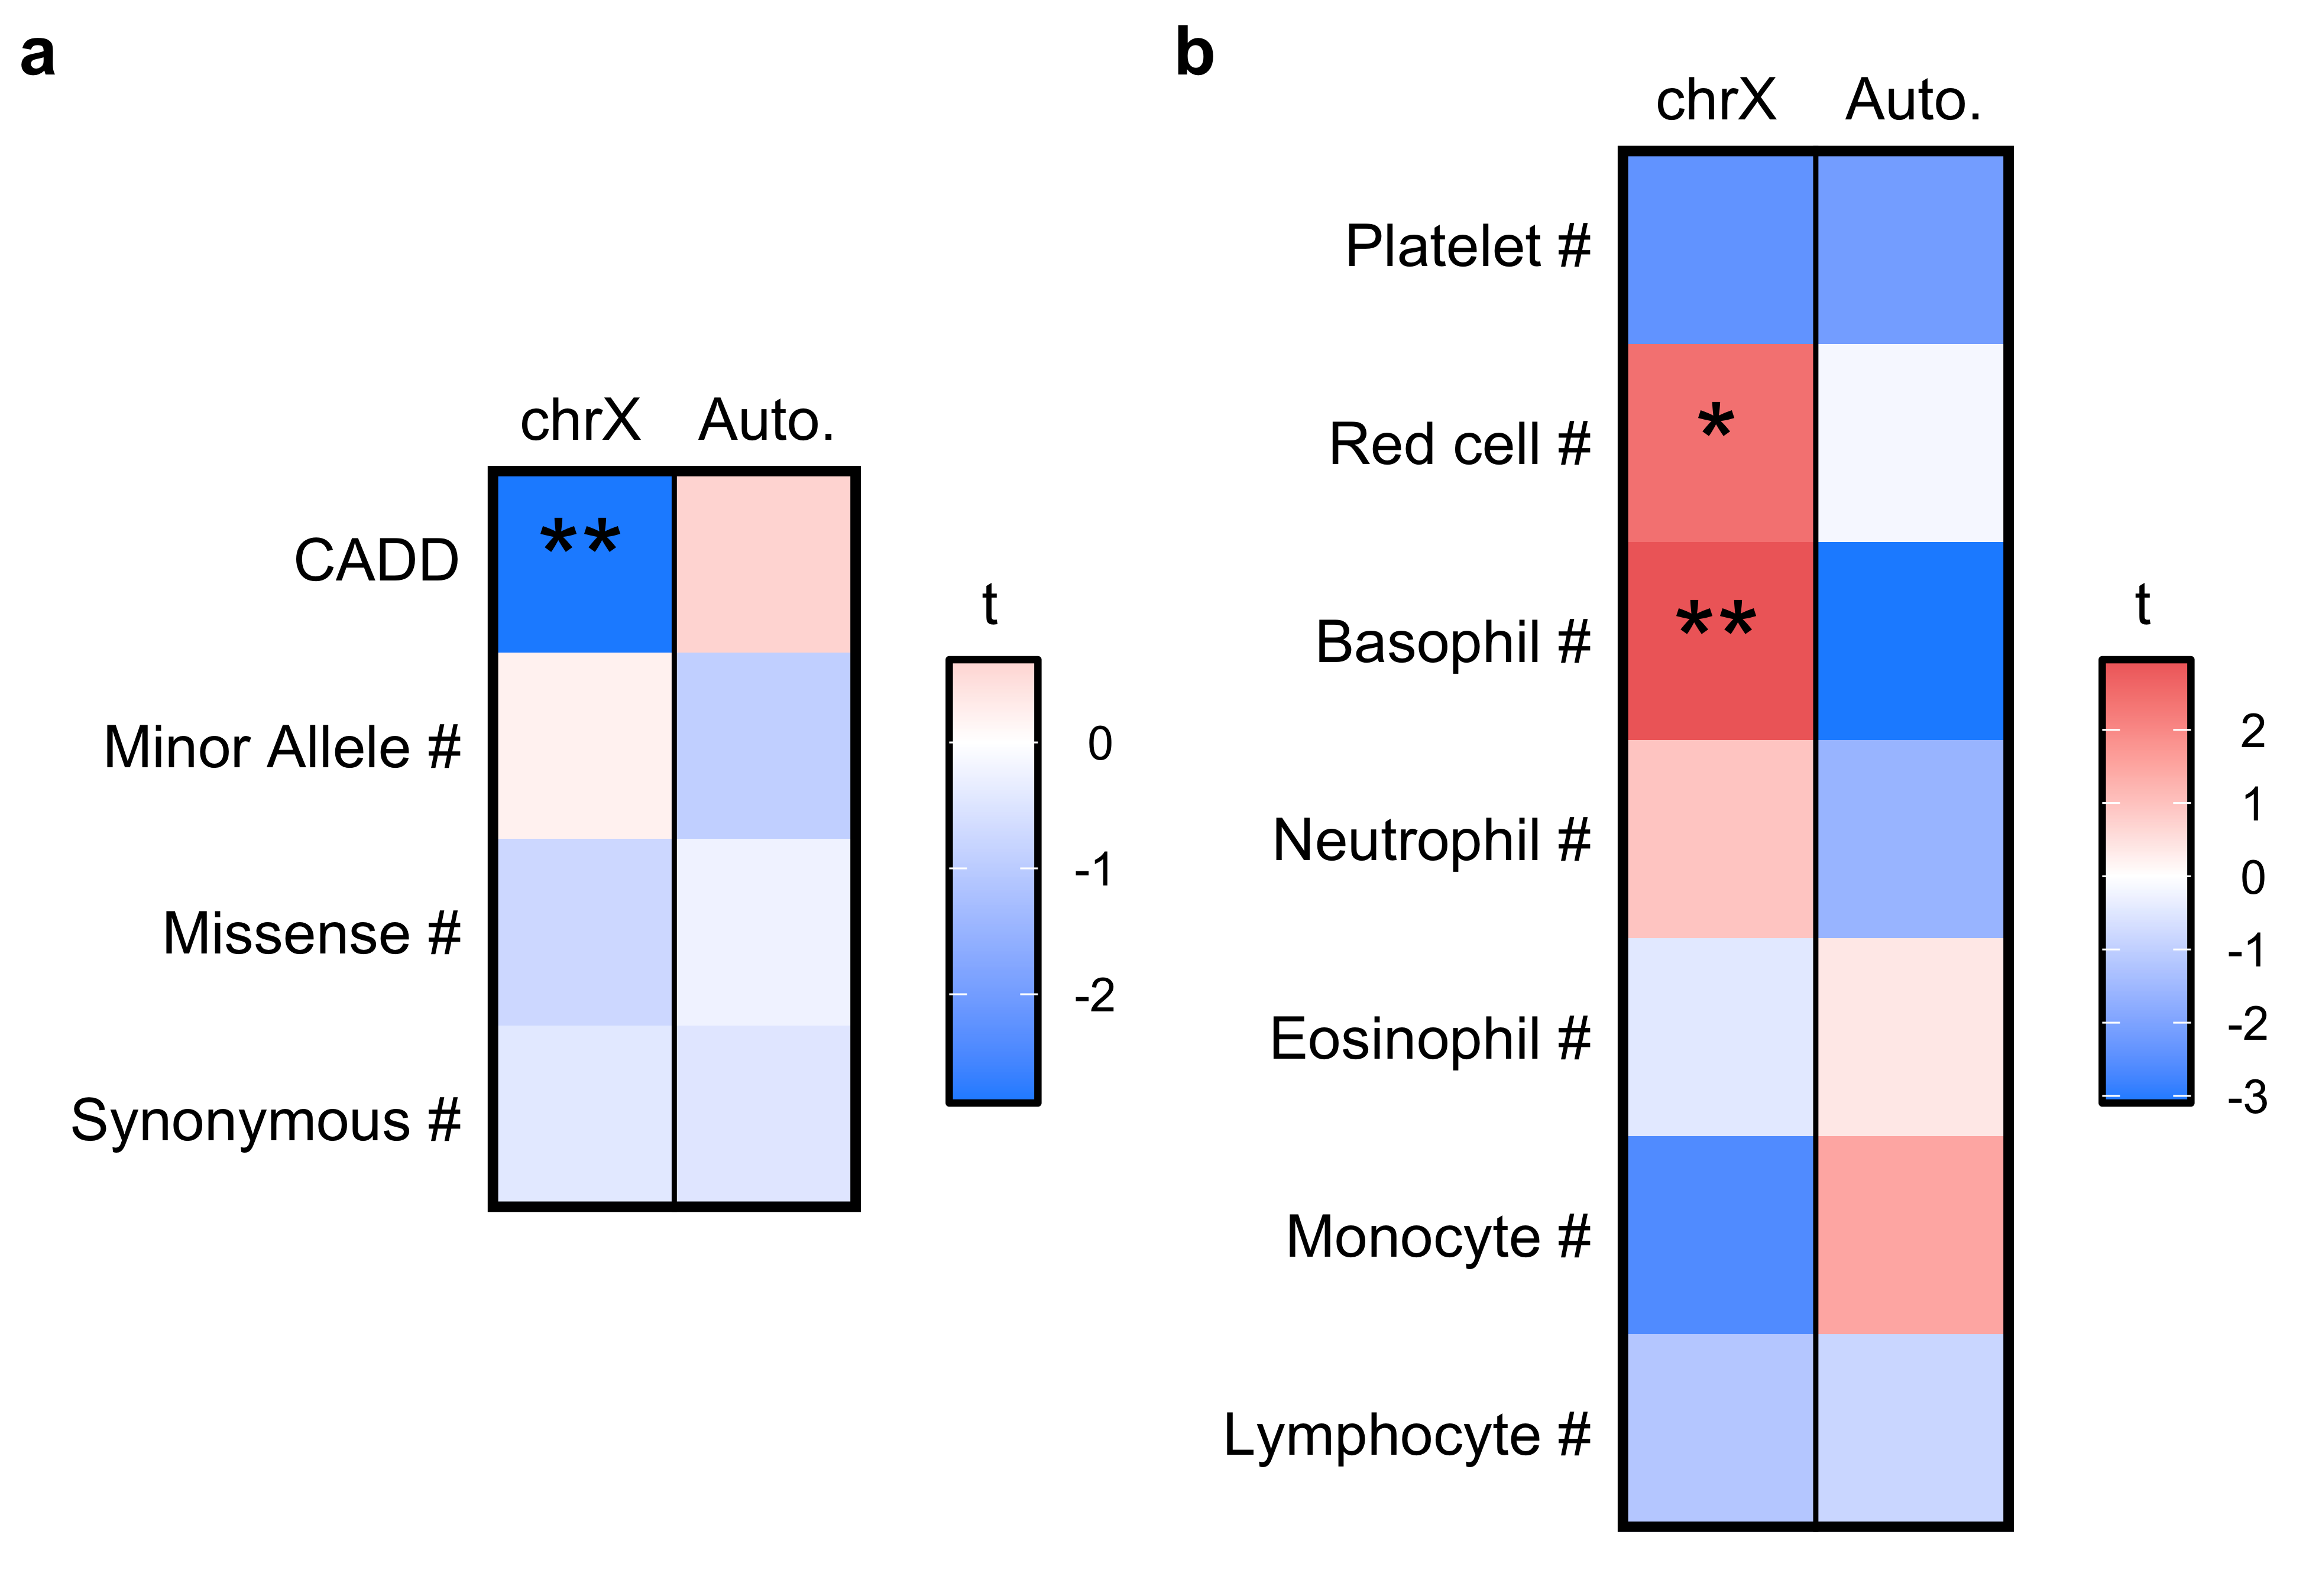
\includegraphics[width=0.5\textwidth]{chapter4/Figures/Figure_2.png}
    \caption{
        Association between genetic scores and skew estimated from expression at heterozygous sites on X chromosome (chrX) and non-acrocentric autosomes (Auto.). Colors indicate the relative t-score from a linear mixed model association test with an asterisks (*) indicating significance at $\alpha=0.05$ and double asterisks (**) indicating significance after Bonferroni correction.
        \textbf{a}, Association results of genetic burden scores with estimated skew. A one-sided t-test was performed under the assumption that increased genetic burden decreases skew towards the haplotype. CADD indicates difference in mean CADD score of each haplotype. The remaining scores compare the number of the indicated mutations on each haplotype.
        \textbf{b}, Association results of proliferative polygenic scores with estimated skew. Counts of different blood cell types were used as a proxy for proliferative potential. A one-sided t-test was performed under the assumption that increased proliferation genetic scores will increase skew towards the haplotype.}
    \label{fig:fig4.2}
\end{figure}